\documentclass[tikz,border=4pt]{standalone}

\usepackage[scaled=0.95]{helvet}
\renewcommand{\familydefault}{\sfdefault}
\usetikzlibrary{arrows.meta,positioning}

\definecolor{Ink}{HTML}{172033}
\definecolor{Muted}{HTML}{596579}
\definecolor{DataFill}{HTML}{E8EDF3}
\definecolor{DataEdge}{HTML}{53657A}
\definecolor{ProcessFill}{HTML}{DCEFEA}
\definecolor{ProcessEdge}{HTML}{23766C}
\definecolor{ModelFill}{HTML}{FCE8D6}
\definecolor{ModelEdge}{HTML}{C66B2B}
\definecolor{OpticsFill}{HTML}{E5EEDB}
\definecolor{OpticsEdge}{HTML}{668348}

\tikzset{
  flow/.style={-{Latex[length=1.8mm,width=1.25mm]}, draw=Ink, line width=0.8pt},
  group/.style={draw=ProcessEdge, fill=white, rounded corners=1.4pt, line width=0.8pt},
  modelgroup/.style={draw=ModelEdge, fill=white, rounded corners=1.4pt, line width=0.8pt},
  data/.style={draw=DataEdge, fill=DataFill, rounded corners=1.2pt, line width=0.8pt,
    align=center, font=\sffamily\fontsize{7.2}{8.3}\selectfont, inner sep=2.2pt},
  process/.style={draw=ProcessEdge, fill=ProcessFill, rounded corners=1.2pt, line width=0.75pt,
    align=center, font=\sffamily\fontsize{7.0}{8.0}\selectfont, inner sep=1.8pt},
  learned/.style={draw=ModelEdge, fill=ModelFill, rounded corners=1.2pt, line width=0.75pt,
    align=center, font=\sffamily\bfseries\fontsize{7.0}{8.0}\selectfont, inner sep=1.8pt},
  optics/.style={draw=OpticsEdge, fill=OpticsFill, rounded corners=1.2pt, line width=0.8pt,
    align=center, font=\sffamily\fontsize{7.0}{8.0}\selectfont, inner sep=2.0pt},
  grouptitle/.style={font=\sffamily\bfseries\fontsize{7.2}{8.2}\selectfont, align=center},
  groupnote/.style={font=\sffamily\fontsize{6.2}{7.0}\selectfont, text=Muted, align=center},
  legend/.style={font=\sffamily\fontsize{6.4}{7.2}\selectfont, text=Muted, anchor=west},
}

\begin{document}
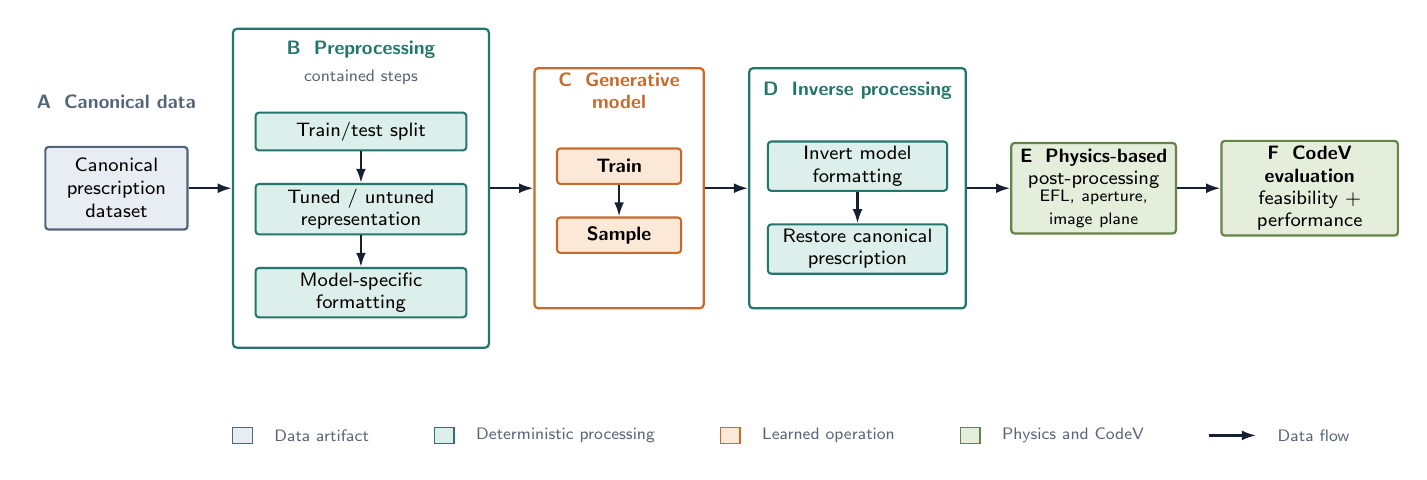
\begin{tikzpicture}[node distance=5.5mm]
  % Outer stages use one fixed relative gap, measured border-to-border.
  \node[data, text width=1.65cm, minimum height=1.05cm] (canonical)
    {Canonical\\prescription\\dataset};
  \node[group, minimum width=3.25cm, minimum height=4.05cm, right=of canonical] (pre) {};
  \node[modelgroup, minimum width=2.15cm, minimum height=3.05cm, right=of pre] (model) {};
  \node[group, minimum width=2.75cm, minimum height=3.05cm, right=of model] (inverse) {};
  \node[optics, text width=1.95cm, minimum height=1.15cm, right=of inverse] (physics)
    {\textbf{E\; Physics-based}\\post-processing\\[-0.2ex]\fontsize{6.0}{6.8}\selectfont EFL, aperture,\\image plane};
  \node[optics, text width=2.10cm, minimum height=1.15cm, right=of physics] (codev)
    {\textbf{F\; CodeV evaluation}\\feasibility + performance};

  % Stage headings and contained operations are positioned from their parent stages.
  \node[grouptitle, text=DataEdge, above=3.5mm of canonical] {A\; Canonical data};
  \node[grouptitle, text=ProcessEdge] at ([yshift=-2.8mm]pre.north) {B\; Preprocessing};
  \node[groupnote] at ([yshift=-6.3mm]pre.north) {contained steps};
  \node[process, text width=2.55cm, minimum height=0.48cm] (split) at ([yshift=7.2mm]pre.center)
    {Train/test split};
  \node[process, text width=2.55cm, minimum height=0.48cm, below=4.0mm of split] (repr)
    {Tuned / untuned representation};
  \node[process, text width=2.55cm, minimum height=0.48cm, below=4.0mm of repr] (format)
    {Model-specific formatting};

  \node[grouptitle, text=ModelEdge] at ([yshift=-3.0mm]model.north) {C\; Generative\\model};
  \node[learned, text width=1.45cm, minimum height=0.45cm] (train) at ([yshift=2.8mm]model.center) {Train};
  \node[learned, text width=1.45cm, minimum height=0.45cm, below=4.0mm of train] (sample) {Sample};

  \node[grouptitle, text=ProcessEdge] at ([yshift=-3.0mm]inverse.north) {D\; Inverse processing};
  \node[process, text width=2.15cm, minimum height=0.45cm] (modelinv) at ([yshift=2.8mm]inverse.center)
    {Invert model formatting};
  \node[process, text width=2.15cm, minimum height=0.45cm, below=4.0mm of modelinv] (opticsinv)
    {Restore canonical\\prescription};

  % Uniform internal and stage-to-stage flow.
  \draw[flow] (split.south) -- (repr.north);
  \draw[flow] (repr.south) -- (format.north);
  \draw[flow] (train.south) -- (sample.north);
  \draw[flow] (modelinv.south) -- (opticsinv.north);
  \draw[flow] (canonical.east) -- (pre.west);
  \draw[flow] (pre.east) -- (model.west);
  \draw[flow] (model.east) -- (inverse.west);
  \draw[flow] (inverse.east) -- (physics.west);
  \draw[flow] (physics.east) -- (codev.west);

  % Relative, evenly separated visual key.
  \coordinate (legendstart) at ([yshift=-11mm]pre.south west);
  \node[draw=DataEdge, fill=DataFill, minimum width=2.5mm, minimum height=2.0mm, inner sep=0pt,
    anchor=west] (ldata) at (legendstart) {};
  \node[legend, right=1.5mm of ldata] (ldatatext) {Data artifact};
  \node[draw=ProcessEdge, fill=ProcessFill, minimum width=2.5mm, minimum height=2.0mm, inner sep=0pt,
    right=7mm of ldatatext] (lprocess) {};
  \node[legend, right=1.5mm of lprocess] (lprocesstext) {Deterministic processing};
  \node[draw=ModelEdge, fill=ModelFill, minimum width=2.5mm, minimum height=2.0mm, inner sep=0pt,
    right=7mm of lprocesstext] (lmodel) {};
  \node[legend, right=1.5mm of lmodel] (lmodeltext) {Learned operation};
  \node[draw=OpticsEdge, fill=OpticsFill, minimum width=2.5mm, minimum height=2.0mm, inner sep=0pt,
    right=7mm of lmodeltext] (loptics) {};
  \node[legend, right=1.5mm of loptics] (lopticstext) {Physics and CodeV};
  \coordinate[right=7mm of lopticstext] (lflowstart);
  \coordinate[right=6mm of lflowstart] (lflowend);
  \draw[flow] (lflowstart) -- (lflowend);
  \node[legend, right=1.5mm of lflowend] {Data flow};
\end{tikzpicture}
\end{document}
